\chapter{Building Scalable Tools}
\label{chap:building-scalable-tools}

\begin{figure}[h]
\begin{tabular}{l r}
\hspace{-1cm}\begin{minipage}{.85\textwidth}
\begin{quote}
{\em Software Engineering might be science; but that's not
what I do.  I'm a hacker, not an engineer.} \\
-- Jamie Zawinski\index[names]{Zawinski, Jaimie}
\end{quote}
\end{minipage}
&

\raisebox{-.8\height}{
	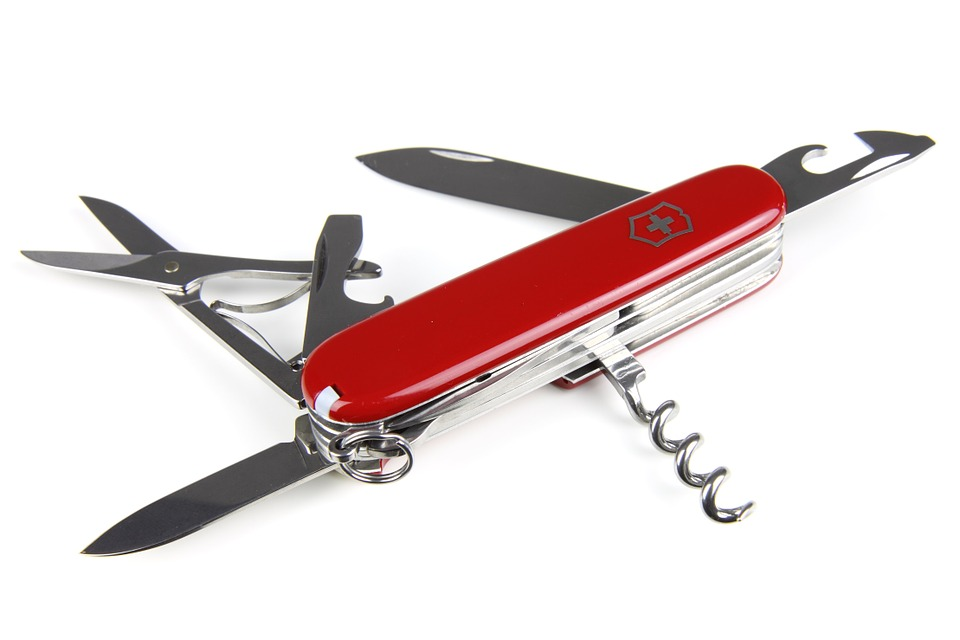
\includegraphics[width=.25\textwidth]{09/pics/army-knife} }

\end{tabular}

\label{fig:army-knife}
\end{figure}

\section{Introduction}
\label{building-scalable-tools:introduction}

In the previous chapter, we talked about our desire to
automate any conceivable task, and we gave examples
ranging from a very simple script building a piece of
software to complex systems orchestrating changes
across thousands of machines.  All of these have one
thing in common: they are software written by system
administrators.  Even though many sysadmins may not
think of themselves as software developers, we all end
up writing our fair share of it.

The programs we create are in many ways different from
a typical software project like a word processor or
similar standalone applications.  System
administrators frequently refer to their tools as
``duct tape''; they tend to consist of little helper
tools, of glue scripts, small programs that are used
to interface with each other, with more complex
software systems, or simply intended to munge data into
a new format.  They often present a simple
command-line interface and operate on plain text
input.

These system tools usually consist of no more than just a
few hundred, rarely up to a few thousand lines of
code. In other words, they're comparatively small, and we
think of them as ``simple'', even as we take pride in
the solutions we've come up with and the automation
they provide us with. 

In this chapter, we will look at how system
administrators develop software, building on the
concept of evolving software as illustrated in the
previous chapter (see Figure
\ref{fig:automation:tools-evolution}).  We begin by
outlining a distinction between ``scripting'',
``programming'' and full fledged software product
development before we present ways of improving our
tools and methods that allow us to build system
components which can be used with the same confidence
we have in the common utilities included in the
operating system.  Approaching automation with these
principles in mind, we will be able to create
solutions that scale with our requirements, and even
though in this chapter we will keep our focus on small
to medium sized programs, we will apply lessons
learned from the profession of software engineering as
well as our own experience as advanced users with a
deep understanding of how our systems (ought to) work.
\\

One of the key insights you can gain from years of
working in different environments, on different
operating systems, and using software tools written by
many different people with many different programming
styles or philosophies is the value of {\em
simplicity} and {\em flexibility}.  The best and most
reliable tools are those that we do not have to think
a whole lot about, the ones we use day in and day out,
and that we can combine with other tools in ways not
predicted by the original author of the software.

As system administrators, we strive to create equally
reliable tools; as software developers (albeit not in
title), we understand and appreciate the Unix
Philosophy\index{Unix!Philosophy}.  We are aware of
the differences in our anticipated user base, as well
as of the fact that we {\em cannot} predict all
possible uses of our software.  This chapter covers
all of this as well as a few general design
principles.  Even if you do not currently think of
yourself as somebody who writes a lot of software,
internalizing these lessons may help you understand
the decisions behind software you already use on a
regular basis and hopefully will help you build better
tools yourself in the future.

\section{How Software evolves}
\label{building-scalable-tools:how-software-evolves}

Software is a curious thing.  Brought into existence
by its creator as a stream of ones and zeros, it
quickly takes on a life of its own.  Software seldom
remains unchanged: bugs are identified and fixed, new
features are added, and previous behaviour changed or
discarded altogether.  All the while, software remains
uniquely reflective of its creator and current
maintainer.  Each person has their own style, and
asking two people to write the same program usually
produces two very different results, even if both may
follow the same requirements or behaviour.

Writing software is hard, in part because we are
effectively unbound by constraints.  Existing software
can be changed; what does not yet exist, can be
created.  Job descriptions for positions in system
administration usually include a required familiarity
with some ``scripting languages'', suggesting that we
do not write software to produce full featured
products.  What we create is often regarded as
``just a script'', a little program, a tool we put
together to automate a workflow.

But {\em simple} does not mean {\em unimportant}.  If
our little tool is actually useful, it will quickly
sprout new features, adapt to being used in other
environments and by different people, integrated into
routine tasks, and eventually relied upon.  Software is
alive; it grows and ultimately escapes your control.
Scripts become programs, which in turn become
infrastructure components or stand alone software
products.

Even though the boundaries between them are fluid, we
can identify an evolution of three approaches to
creating software: scripting, programming, and formal
software development.  It is important to understand
the difference in scope, usability, and implications
resulting from each approach.  Being aware of which
step on the latter you find yourself allows you to
more clearly understand the requirements and
appropriate solutions.  Let us look at these three
stages in more detail.

\begin{sidenote}
{\bf ``Scripting Languages''} \\

It is worth noting that we use the terms ``script''
and ``program'' (both as nouns or as verbs) in a
rather language agnostic manner.  ``Shell scripts''
are often a collection of commands with limited
control flow, most commonly written using
Bourne(-like) shell syntax.  They tend to evolve out
of actual command pipelines executed interactively,
combining the common Unix tools such as {\tt
awk(1)}\index{\tt awk(1)}, {\tt grep(1)}\index{\tt
grep(1)} or {\tt sed(1)}\index{\tt sed(1)}. \\ [10pt]

A number of general purpose programming languages that
are sometimes referred to as ``scripting
languages''\index{Scripting Languages} facilitate the
development of quick prototypes due to a number of
features such as being interpreted from source code
(versus a compiled language), having extensive support
for file system interfaces, requiring little
structure, and being intuitive to use.  Perl, Python,
or Ruby are often cited as examples of ``scripting
languages''. \\ [10pt]

But it is dangerous to make the mistake of calling
something a ``script'' just because it was written
using a given language.  It is certainly possible to
create complex programs in shell, just as it is
possible to write the most simplistic scripts in, say,
Python.  And while you can write full-fledged,
reliable and scalable products in Perl or Ruby, using
any one language does not impart code maturity or
superiority upon your solution.  Our discussion of
these terms focuses on how we choose to approach the
development process and the resulting implications on
the user interface and robustness of the tool in
question, not the language in which it was written. \\
[10pt]

Describing a ``scripting language'' as aiding in the
development of a {\em prototype} is more useful in the
definition of what a ``script'' is than what the
language itself is capable of.  Outside of the
customization of your own environment, scripts are
most useful to rapidly develop a program prototype, a
proof of concept, a first stab at figuring out how to
solve a problem programmatically.  From this prototype
evolves, eventually, a more robust program, which may
be written in the same, or a different language..
\end{sidenote}


\subsection{Scripts}
\label{building-scalable-tools:how-software-evolves:scripts}

``Scripts'' are primarily defined by the language we
use to describe them: we ``throw together a quick
script'', or we ``whip up a few lines of shell code''.
The results reflect this attitude.  Our scripts are --
initially anyway -- not more than a collection of
commands, stored in a file to save us the hassle of
having to remember and type them repeatedly.  Our code
example in the previous chapter (Listing
\ref{code:automation:gcc}) is a good illustration of
this approach.  As a simple solution to a problem we
don't anticipate to be used by other people, we make a
number of assumptions about the user's environment,
the invocation, user input, and so on.  All of these
assumptions tend to be implicit or hidden, and we only
become fully aware of them when they no longer hold
and the program misbehaves.

Scripts tend to be used for very simple tasks, and
they often rely heavily on the environment.  Spanning
just a few dozen lines or so, they expect certain
variables to be set, a directory hierarchy to follow a
specific layout, or they may attempt to write to files
in the current working directory.  Due to a lack of
error checking, online help or documentation, they
often really are only suitable for use by the person
who wrote them.

These little helper scripts may start out as shell
aliases or functions, or are stored in a private
directory in one's {\tt PATH} and used primarily to
customize your own environment and automate a few of
your most common tasks.  But if what we whipped up
there is actually useful, it will invariably evolve
into a larger program.  With every additional user, it
will grow new features, assumptions about the
environment it executes in will be removed or turned
into assertions.  We may add command-line option
parsing, explicit error checking and reporting, fix
bugs, and increase overall robustness.  Before you know
it, what started out as a few dozen commands stashed
away in a file somewhere becomes a reliable program.

\subsection{Programs}
\label{building-scalable-tools:how-software-evolves:programs}

All but the most simple scripts see some ongoing
development as their user base increases.  Frequently
we start out whipping up a script -- there it goes
again, this phrase -- only to come back to it (not
much) later, adding features and extending its
functionality.  In fact, we often throw out our
initial prototype and rewrite the tool, possibly in
another language.  Even though it is difficult to
willingly discard an existing solution into which time
and effort have gone, this is, after all, the the main
purpose of a {\em prototype}: to allow you to learn
the details of the problem and to provide a proof of
concept implementation on which to model your later
program.

In the process of writing a prototype, you will
identify new desirable features, figure out what works
and what doesn't, as well as discover hidden
requirements and dependencies.  Growing in complexity
as well as maturity, a program developed from a
prototype becomes a more reliable tool.

In contrast to simple scripts, programs make use of
common toolkits, software libraries or modules to
combine existing frameworks and implement new
functionality. They provide a more consistent
interface, account for differences in the environment
and may be able to handle larger input data, for
example.  Programs range from a few hundred to a few
thousand lines of code; they may consume or provide an
\gls{api} to a service and interface with various other
components without human interaction.

Programs and scripts are, for the most part, what many
of us System Administrators are creating when we write
software. We put tools together that range from
trivial to moderately complex, targeting as our
intended users people like us, our peers, possibly
other people within our organization but rarely
outsiders with entirely different environments or
requirements.

System administrators are known to half-jokingly refer
to themselves as duct tape slingers, experts in
stringing together systems and programs in ways
previously unimagined and perhaps unintended; our
tools function as glue, to bind together independent
system components.  But here, too, the language we
choose reflects the attitude we have towards our
tools, and using the proper terms helps develop
greater confidence and a sense of pride in our
creation.

What began as a set of simple scripts may have
developed into a number of complex programs used
across numerous systems.  Without realizing, we may
have developed a core infrastructure component upon
which our organization relies.  At this point, the
software is likely to have advanced to into the stage
of being a full-featured, self-contained application,
requiring ongoing maintenance, development and
support.  We have crossed the boundary from
``program'' to product, often without being aware of
it.

The larger our infrastructure grows, the more complex
become the programs we use to hold it together.  At
some point, we need something stronger than duct tape.
That is, we need to change our attitude to treat the
software we create on this particular layer of the
infrastructure ecosystem as requiring -- deserving --
a more professional approach.

\subsection{Software Products}
\label{building-scalable-tools:how-software-evolves:software-products}

On the far end of the spectrum of software evolution
from a simple script or prototype lie complete,
self-contained ``products''.  Typical examples from
outside the world of System Administration might
include a word processor with a graphical user
interface, a music player, a multi-user game, or
perhaps a mobile app.  The range of what these
applications do is unbound, but what they have in
common is that we regard them to be, by and large,
self-contained.   We often use words such as
``polished'', or ``full-fledged'' to express a certain
level of professionalism or completeness.

We imagine a team of software developers creating such
a product with a clear vision of features,
requirements, specifications, and measurable goals all
following good and sound software engineering
approaches.  We envision product meetings, heated
discussions around implementation details and
algorithms, concentrated developers scribbling away on
a whiteboard and user-interface experts designing what
the application will look like.  We certainly do not
think of these products as ``whipped up'' in an
afternoon, or even over the course of a week or two.

But consider some of the software we use routinely,
such as a configuration management system or a package
manager.  Despite being self-contained, large,
complex, and far from being a small little program or
a collection of scripts, these software products
frequently {\em did} evolve out of smaller components,
initially written by system administrators to, as they
say, ``scratch an itch'', to solve a very specific
problem encountered by the author.  As noted before,
the distinctions between different types of software
are far from clear cut, and system administrators may
well become ``system engineers'' or ``system
programmers'' and shift their primary focus on the
development of such products.

Full products require a dedicated team of engineers to
not only write the code or to add features, but to
provide the necessary support and maintenance of the
product throughout its life cycle:  it is commonly
estimated that the \gls{tco}\index{Total Cost of
Ownership} of any software product consists to
approximately 75\% of ongoing maintenance and bug
fixes!\footnote{System Administrators tend to agree
that installation and operational maintenance of the
product make up the remaining 75\%.}

But even though system administrators may well play an
important role in the design of internal
infrastructure components and applications, we will
focus on the development of smaller tools and more
typical system utilities in this chapter.  Even if you
end up building more complex software components,
hopefully you will find some useful information in the
following sections.

\begin{sidenote}
{\bf Open Source as Quality Assurance} \\

Companies nowadays routinely release many of their
system tools as Open Source\index{Open Source}, often
benefitting significantly from outside feedback and
contributions.  However, as a pre-requisite to being
adopted by others, these programs already tend to
exhibit many of the desirable features we describe
later in this chapter.  This is partially a result of
good programming practices inside the company or by
the engineers in question, but another significant
factor is the fact that any open sourced program
reflects directly on the authors and organization with
which it is associated. \\ [10pt]

As a result, programs released to the world often
undergo significant additional scrutiny, detailed code
reviews, and developers are asked to provide useful
documentation alongside the product.  All of these
things should of course be mandatory for internal
tools as well, but for internal releases they are easy
to neglect.  Paradoxically, we are often willing to
bet our infrastructure, our product, and our business
on software we are afraid might be criticized in
public.  Ruslan Meshenberg noted in 2012: \\ [10pt]

``{\em [At Netflix] We've observed that the peer
pressure from `Social Coding' has driven engineers to
make sure code is clean and well structured,
documentation is useful and up to date.  What we've
learned is that a component may be `Good enough for
running in production, but not good enough for [Open
Source].' ''}
\cite{building-scalable-tools:netflix-open-source} \\
[10pt]

With this in mind, it behooves us to develop {\em all}
of our software with the intention of making it
public.  The prospect of releasing our code as Open
Source to the world will aide as a significant Quality
Assurance factor.
\end{sidenote}



\section{Principles of Developing Robust System Tools}
\label{building-scalable-tools:principles}

A large number of of System Administrators remain --
unconsciously and unintentionally -- stuck in
``scripting mode''.  That is, their software reflects
the mindset and language previously described, and the
resulting tools are at times lacking in reliability or
portability, even though they may work well in the
specific environment they were developed in.  But
today's infrastructures are growing exponentially in
size and complexity, and we often find that what used
to be ``good enough'' isn't any longer.

One of the most important methods of improving this
status quo is to change how we view our own software
tools.  In order to improve stability, reliability,
portability (and thus flexibility and scalability), we
need to stop distinguishing our tools from those
provided by the operating system or other providers.
We should hold the software we write to the same
standards in terms of quality, usability, and
documentation as any other product.  In other words:
always write your tools such that they could be widely
distributed, as if they were core components of your
OS distribution.

With this approach, you will observe a shift in focus
away from solving just your own, very specific problem
in your own, unique environment towards creating
general solutions.  This allows you to continue to use
or adapt your tools as your infrastructure changes.
\\

In this section, we will discuss a number of
principles that will guide you in this change of
viewpoints and development practices.  You may already
be familiar with some of them, as we may have
mentioned them previously in this book, while others
are common recommendations for any type of
professional software development.

For example, the Python programming language includes
as a so-called ``easter egg'' its own programming
philosophy, known as the ``Zen of Python''\index{Zen
of Python}, which we show in Listing
\ref{code:zen-of-python}.  Throughout this chapter, we
will reference parts of the Zen of Python, and you
will find that it applies equally well to other
programming languages and software development
principles.

As you read on, try to think about how you would apply
the principles discussed here to your own software.
That is, do not regard them as rules or guidelines for
large scale software development only, but as general
advice applicable also and {\em especially} to
small(er) system tools.  You will be able to identify
many of them as underlying the programs and utilities
you already use on a daily basis, and hopefully begin
to view your own software as no different.

\begin{lstlisting}[float,basicstyle=\tiny,label=code:zen-of-python,caption={[The
Zen of Python]Sound programming advice that transcends
language specifics.}]
$ echo "import this" | python
The Zen of Python, by Tim Peters

Beautiful is better than ugly.
Explicit is better than implicit.
Simple is better than complex.
Complex is better than complicated.
Flat is better than nested.
Sparse is better than dense.
Readability counts.
Special cases aren't special enough to break the rules.
Although practicality beats purity.
Errors should never pass silently.
Unless explicitly silenced.
In the face of ambiguity, refuse the temptation to guess.
There should be one-- and preferably only one --obvious way to do it.
Although that way may not be obvious at first unless you're Dutch.
Now is better than never.
Although never is often better than *right* now.
If the implementation is hard to explain, it's a bad idea.
If the implementation is easy to explain, it may be a good idea.
Namespaces are one honking great idea -- let's do more of those!
$ 
\end{lstlisting}


\subsection{Unix Philosophy and User Interface}
\label{building-scalable-tools:principles:unix-philosophy-user-interface}
\index{Unix!Philosophy}

One of the most important aspects of any tool you may
write is its user interface.  The way in which the
program is invoked and interacts with its users
determines whether or not it can become a core
component of the system administrator's toolkit, if
it remains a special purpose utility, if it will be
forgotten, unused, or cursed.  Many different
factors define the user interface, but the most
dominant convention for robust and scalable tools
here remains the ubiquitous Unix Philosophy:

\begin{quote}
Write programs that do one thing and do it well. Write programs to work
together. Write programs to handle text streams, because that is a
universal interface.\cite{building-scalable-tools:mcilroy-unix-philosophy}
\end{quote}

We already discussed this elegant and succinct
definition early on in this book.  Now it would be
silly for us to repeat here all the fine text from our
earlier chapter, so why don't you go ahead and flip
back to Section \ref{unix:philosophy} and reread it --
it won't take too long!  (Reuse of modular components
to avoid duplication of code is, incidentally, also
sound programming advice; we hope it translates
equally well to writing.)

Entire books have been written on this approach to
programming and tool design, several of which are
considered must-reads for any system administrator or
software engineer
(\cite{building-scalable-tools:kernighan-pike-practice},
\cite{building-scalable-tools:kernighan-pike-upe}, and
\cite{building-scalable-tools:esr-taoup} are certainly
among them), but let us review the three key aspects
of the Unix Philosophy here as well.  The discussion
of software development principles within system
administration wouldn't be complete without.

\subsubsection*{Simplicity}
\index{Simplicity}

{\em Write programs that do one thing and do it well.}
Design your tools to be as simple as possible.
Writing software is {\em hard}!  The more
functionality you attempt to implement, the more code
you have to write, and more code inevitably translates
to more bugs.  Given this widely accepted
understanding, shouldn't it be easy to write {\em
simple} tools, to eschew the added complexity of
additional non-essential features?  Unfortunately,
identifying only the necessary features and
restraining oneself from adding functionality can be
quite difficult.

In order to write a program, we have to understand the
problem we're trying to solve well enough to be able
to {\em explain it to a computer}.  The more we think
about a problem, the more corner cases we discover,
the more features we envision as useful, and as we
write our code, we begin to expand the scope of the
program.  The more users our tool has, the more
requests we get to implement new features as well.
Within the Software Engineering discipline, this
phenomenon is known as "creeping features", and it
takes a strong mind to keep a project within its
original scope.

When we build software, we are in control.  We
determine exactly how the program will behave, how the
user will interact with it.  Wishing to remain in full
control, we frequently fall into the trap of writing
our own modules or to implement functionality that
exists in other tools, because we grossly
underestimate the time and effort required to do so.
Frequently these other tools don't follow our own
mental model or are inconvenient to interface with,
and reading other people's code, program specification
or documentation is very difficult -- and no fun!

All of this leads to increased complexity in the
software we write, and simultaneously tends to
restrict its flexibility, as we impose our own
perception of how to interact with the tool upon our
users.  \\

%An example:  We frequently need our tool to read some sort of input and
%act on it.  Program often need to read a list of hostnames, for example,
%to perform some action against each of the entries found.  As we develop
%our prototype, we immediately begin to add code to accept a
%command-line option specifying the input file and then to process it.
%That is, we need to {\tt open(2)} the file and read the contents.  But a
%number of things can go wrong in this small part already:  the given file
%might not exist, or we might not have permissions to open it.  So we add
%explicit error checking and meaningful error messages.
%
%While any competent programmer can write the required code for this
%without much effort, ask yourself whether or not this is really
%necessary.  Suppose your tools simply required input to be given on {\tt
%stdin}?  Not only would you gain flexibility -- your program can now take
%input from another program without any intermediary files -- but now file
%I/O and all the many things that can go wrong with it are no longer your
%problem.  Instead, we let the shell do all the heavy lifting here.
%
%Let's look at the seemingly trivial difference in invocation.  If we
%accept input only from a file, then we are not able to use common tools
%like {\tt awk(1)}, {\tt grep(1)}, or {\tt sed(1)}, for example, to
%process the input before feeding it to our command.  Instead, we need to
%first prepare the input in a file.  If our tool accepts input from {\tt
%stdin}, on the other hand, we can easily use it in much the same way we
%use almost any other Unix tool.
%
%\begin{lstlisting}[float,label=code:invocation-file-input,caption={Comparison
%of common use cases when reading input.}] $ generate-hostlist > hostlist
%$ generate-hostlist | mytool $ mytool -f hostlist              $ mytool
%<hostlist $ grep pattern hostlist >file     $ generate-hostlist | \ $
%mytool -f file                            grep pattern | mytool
%\end{lstlisting}
%
%Note that you have not lost any functionality: if you want to avoid
%having to run the command to generate the input, you can still read data
%from a file via the shell's  input redirection mechanism ({\tt <}).  At
%the same time, however, you can {\em also} read data from another tool
%via a pipe.  By simplifying, your tool has become more reliable (you have
%eliminated the possibility of any bugs in your file I/O handling
%routines) but simultaneously {\em more flexible}.
%

As we develop scalable system tools, we strive to
simplify code, interfaces, and logic as much as
possible, but we need to remain aware that certain
parts may remain complex (albeit not {\em complicated}
or {\em convoluted}!).  That is, at some point a tool
cannot be simplified any further:  Any program you
write has what Fred Brooks\index[names]{Brooks Jr.,
Frederick P.} terms ``essential
complexity''\index{complexity!essential} as well as
``accidental
complexity''\cite{building-scalable-tools:brooks-mmm}.\index{complexity!accidental}
{\em Essential complexity} is inherent to the task the
software performs and cannot be reduced; {\em
accidental complexity} depends on how we implemented
the tool.  For example, the ability of many of our
tools to be able to process input one line at a time
might be {\em essential complexity}, but implementing
file I/O (and handling well all the various failure
scenarios in doing so) would be {\em accidental
complexity}: you'd most likely be better off simply
reading input from {\tt stdin}.

%In our previous example the ability to process text
%input one line at a time and perform whatever action
%the tool was built to perform is essential
%complexity, while adding logic and code to handle
%file I/O with all its error scenarios is accidental
%complexity.
%
Applying this concept of identifying and only writing
the code that you really need to while reducing the
(accidental) complexity of both the interface as well
as the implementation lies at the heart of the Unix
philosophy, and is echoed in the Zen of Python:

\begin{quote}
Simple is better than complex. \\
Complex is better than complicated.
\end{quote}

\subsubsection*{Tools as Filters}

As the author of a program, we consider ourselves the
ultimate authority on how it might be used.  We define
the interfaces of our tools, and thereby prescribing
possible usage.  But is is important to realize that
we cannot possibly foresee all the ways in which our
program may be used.  Any program we write may end up
being utilized in ways {\em not} anticipated by us.

The advice to {\em write programs to work together}
embodies this awareness.  Because we cannot know how
users will take advantage of the functionality our
program provides we need to allow them to combine it
with great flexibility.  Since you cannot presume all
use cases, begin by writing your tools such that they
accept input from {\tt stdin} and generate output to
{\tt stdout}.  As shown above, this allows you to
simplify your program by eliminating all the
comlexities of file I/O for these cases.  But what's
more important: your tool can now be used as a {\em
filter}.  Your users gain significant flexibility, as
they can now combine other tools to prepare input for
or post-process output from your program with great
ease.

This approach leads to a few practical considerations.
For example, it is often a good idea to process input
in chunks (most commonly one line at a time) rather
than attempt to store all input in a data structure
before handling it.  This allows you to handle
arbitrarily large input, as you are not bound by the
amount of available memory.  Your program will also
become more responsive, as the user won't have to wait
for all input to be read before your program can begin
processing it.\footnote{Of course there are
exceptions: certain programs require all input to be
present before they can produce a result (the {\tt
sort(1)}\index{\tt sort(1)} utility is one such
example), but as a general rule of thumb line-based
processing of input data makes for a simpler approach
and a more useful filter.}

Treating your program as a filter also forces you to
make a very explicit distinction between the desired
output it produces and any error- or diagnostic
messages it may generate.  Since the expected output
may need to be further processed by other commands,
Unix tools have a long tradition of printing such
notifications to {\tt stderr}, allowing you to process
the valid output generated while at the same time
displaying errors to the user.

Likewise, do not assume that your program is invoked
interactively.  That is, you cannot require input from
the user.  For example, it is a common mistake to
prompt the user for confirmation of certain actions
(``Continue? (y/n)'').  To make matters worse,
inexperienced programmers often attempt to read a
response from {\tt stdin}:  if your program is used as
a filter in a pipe, then {\tt stdin} contains the data
it is supposed to consume and cannot be used for
interactions with the user!

In cases where interactions with the user cannot be
avoided, your program should read input from the
controlling terminal directly (via {\tt /dev/tty} or
the terminal identified via the {\tt
tty(1)}\index{\tt tty(1)} command or {\tt
ttyname(3)}\index{\tt ttyname(3)} library function),
but be aware that any interactive usage blocks the
entire pipe until the user has provided the required
input.  Unix tools that allow for interactive use
often have an explicit command-line switch to turn
this behaviour on (commonly {\tt -i}) or off
(commonly {\tt -f}), and you may wish to consider
following that convention.

Finally, you should carefully evaluate the error
conditions under which your program terminates.  As a
filter, it is not uncommon to process large amounts of
input and have many other tools depend on the output
you generate.  If your program aborts upon
encountering any error condition, the entire pipe is
interrupted.  For example, if your program expects
input to be in a certain format, aborting if data does
not conform to this format may be a bad idea.
Instead, it might be desirable to instead issue a
warning (on {\tt stderr}) and proceed to the next line
of data.

This behaviour is an application of what is known as
the {\em Robustness Principle}\index{Robustness
Principle}, also known as {\em Postel's
Law}\index[names]{Postel, Jon}\index{Postel's Law},
described in an early specification of TCP:

\begin{quote}
Be conservative in what you do, be liberal in what you
accept from
others.\cite{building-scalable-tools:postel}
\end{quote}

That is, your program should tolerate malformed input,
but produce well-defined output.  Note, however, that
it is a common misinterpretation of Postel's Law to
suggest that a program should always try to {\em
process} all input as if it was valid, even if it is
not.  This can be dangerous, as acting on malformed
input can lead to a number of security problems, such
as e.g. accidental code execution as a result of
interpreting or evaluating input in an executable
context.  Proper input validation is still required;
it may be sufficient for your tool to warn the user on
invalid input before moving on to the next chunk of
data rather than aborting altogether.

\subsubsection*{Text Streams}

\begin{lstlisting}[float=t,label=code:grep-/etc/rc.conf,caption={[{\em
rc(8)} key=value pair configuration]The BSD {\em
rc(8)} system uses simple key=value pairs as a means
of configuration, making it trivial to process using
common Unix tools.\index{\tt apache}}]
$ grep '^[^#].*=' /etc/rc.conf | sort
apache=YES
dhclient=YES
dhclient_flags="xennet0"
hostname=panix.netmeister.org
ip6mode="autohost"
ntpd=YES
postfix=YES
rc_configured=YES
rtsol="YES" 
rtsol_flags="xennet0" 
sshd=YES
syslogd_flags="-snvv"
$ 
\end{lstlisting}


Unix tools have a long tradition of operating on plain
text.  Consider the various commands you use on a
daily basis: {\tt awk(1)}\index{\tt awk(1)}, {\tt
grep(1)}\index{\tt grep(1)}, {\tt head(1)}\index{\tt
head(1)}, {\tt sed(1)}\index{\tt sed(1)}, {\tt
sort(1)}\index{\tt sort(1)}, {\tt tail(1)}\index{\tt
tail(1)}, {\tt uniq(1)}\index{\tt uniq(1)}, {\tt
wc(1)}\index{\tt wc(1)}, ... all of them process data
or generate output by reading and writing text
streams, described by Douglas
McIlroy\index[names]{McIlroy, Douglas} as ``a
universal interface'', and their ubiquity is tied
directly to the use of these tools as filters.

But  data structures frequently are complex
representations of the author's own mental model, and
programs regularly need to translate representations
of data for other tools to process or to retain state
information in between invocations.

Many programming languages allow for {\em
serialization} of objects into a binary representation
that can be read from or written to a file without the
(at times significant) overhead of parsing text,
matching patterns, and reconstructing a complex
object.  This approach, while often the most
efficient, would, however, limit your program's ability
to be combined with other tools.  It could no longer
function as a filter, as any command generating input
would need to produce the specific format required,
and any output could only be processed by tools
capable of understanding this format.

The {\em \gls{xml}}\index{XML} and the {\em
\gls{json}}\index{JSON}, are two examples of data
representation that attempt to strike a compromise
between binary formats and completely unstructured
text streams.  For many system tools, however, text
streams remain preferable, as they provide a
consistent user interface across the environment and
very clearly put the focus on who the primary consumer
of the data is: the user!  The person running the
commands needs to be able to make sense of their
intput and output.  It is preferable to be wasteful
with computing resources and have your program require
a few clock cycles more to process the data than to
waste your users' time and energy, as they try to make
sense of the format.

%This approach translates to configuration files as well: storing them in
%plain text rather than as a bitstream or other opaque format makes it
%possible for the system administrator to read and understand the file, to
%search through it without requiring special tools.  In fact, it is not
%uncommon to generate or process configuration files using other utilities,
%which is why they lend themselves as a good example here.
%
%As long as these representations remain in text rather than binary format,
%they can still be processed using tools that are unaware of the format --
%at least to some degree.  But the more complex the structure of the data
%becomes, the more difficult it is to process data using general purpose
%tools.  For example, we can easily extract simple {\tt key=value} from a
%typical Unix configuration file, as shown in Listing
%\ref{code:grep-/etc/rc.conf}, but a configuration file such as a Mac OS X
%{\em property list} as shown in Listing \ref{code:ipconfiguration.plist}
%requires special purpose tools that are aware of the structure of the
%data.
%
%\begin{lstlisting}[float=b,label=code:ipconfiguration.plist,caption={This
%excerpt from a Mac OS X {\em property list}, describes a host's partial
%network configuration.  Processing it using common Unix tools is less
%straight forward then a simple text file.}]
%<?xml version="1.0" encoding="UTF-8"?>
%<!DOCTYPE plist PUBLIC "-//Apple//DTD PLIST 1.0//EN"
%        "http://www.apple.com/DTDs/PropertyList-1.0.dtd">
%<plist version="1.0">
%<dict>
%[...]
%  <key>IPConfiguration</key>
%  <dict>
%    <key>ConfigureIPv6</key>
%    <true/>
%    <key>DHCPv6RequestedOptions</key>
%    <array>
%      <integer>23</integer>
%      <integer>24</integer>
%    </array>
%    <key>DiscoverRouterMACAddressTimeSeconds</key>
%    <integer>60</integer>
%    <key>Verbose</key>
%    <false/>
%  </dict>
%</dict>
%</plist>
%\end{lstlisting}

In the Unix world, we have a thriving Open Source
ecosystem of tools and libraries; utilities written by
one person or organization are often used and extended
by others, possibly in ways not imagined by the
original author.  A stricter data model imposes
restrictions on how the tool may be used, extended, or
built upon; encoding the structure in the input or
output format aids other programs, while text streams
are helpful for human consumers.  The humility to put
the user before the program, to understand that it is
{\em people} our tools interact with primarily and
whose job they should make easier leads us to favor
text streams.

\subsection{Principle of Least Astonishment}
\label{building-scalable-tools:principles:pola}

As system administrators, we have enough excitement
and unexpected events occurring in our daily life.  We
do not appreciate our tools surprising us.  In fact,
one of the most important features that makes our
preferred tools reliable is the fact that they are
{\em predictable}.  Not only do they perform the task
they were designed to do well, but we can rest assured
that they will behave unsurprisingly under even
unanticipated circumstances.

We already mentioned Postel's Law as sound advice, and
in previous chapters we have discussed {\em
idempotence} as an important property of a reliable
system.  In addition to these traits, and perhaps more
than just being robust and predictable, we want our
tools to be {\em boring}.  Our users should never be
surprised by the outcome of invoking our program, nor
should we attempt to surmise the user's intentions.
This concept is referred to as the {\em Principle of
Least Astonishment}\index{Principle of Least
Astonishment} or \glslink{pola}{POLA}.

Our tool should be explicit and specific in both its
success- as well as error-cases.  When determining
your program's logic, ask yourself what the user would
most likely anticipate the outcome to be.  For
example, if you were to move a file from one partition
to another, the normal outcome is that in the end the
file no longer exists in the first location, but does
in the second.  One approach to perform this task
might be to first open the original file, read its
contents into memory, remove the file, then write the
contents from memory to the new location.  But what if
something goes wrong in the process of writing the
data and you are forced to abort the program?  The
original file was already removed, which would come as
a rather unpleasant surprise to the user.  The
Principle of Least Astonishment would demand that the
file {\em only} be removed from the original location
if the copy was successfully written.

Unfortunately, it is not always this obvious to
anticipate what may or may not surprise your users.
Destructive actions, such as removing or overwriting
files, or discarding input data can lead to
significant frustrations when they occur unexpectedly.
As you write your program, carefully consider the way
you yourself interact with existing, similar tools,
and what your expectations are of them, then translate
this behaviour to your own programs.

\subsection{Explicit and predictable failure}
\label{building-scalable-tools:principles:explicit-and-predictable-failure}

Even though Postel's Law asks us to be liberal in what
we accept, it is often preferable to fail early and
explicitly due to a known error condition rather than
to trot along and run the risk of entering an
undefined state with possibly disasterous
consequences.  Remember, as long as you know there was
an error, you can still control the resulting process
flow and yield predictable outcomes.  This includes
{\em predictable failure}!\index{predictable
failure}\index{failure}

It is imperative that the user can easily determine
whether or not your program succeeded.  But since Unix
tools are often used as filters or building blocks of
larger programs, it is not sufficient to generate an
error message.  Any program building on your tool
would have to parse this output and react to it
accordingly.  Instead, the convention is to indicate
success or failure via an exit code, typically {\tt 0}
on success and any value larger than {\tt 0} if an
error was encountered.  This allows programmatic use
of your tool without the overhead involved in
inspecting text output.  The combination of processing
text streams, of generating error messages to {\tt
stderr}, and to return a meaningful exit code allows
your program to behave predictably and reliably in
success and failure mode equally.

As noted before, the principles which allow us to
build reliable tools are reflected in the Zen of
Python, applying equally to how we may structure our
code as well as how we design our user interfaces:

\begin{quote}
Explicit is better than implicit. \\
In the face of ambiguity, refuse the temptation to guess.
\end{quote}

Create boring tools.  Your users will thank you by
being able to rely on them.

%XXX examples (some tool that returns 0 on errors -- yum?)

\subsection{There's no such thing as a temporary solution.}
\label{building-scalable-tools:principles:no-temporary-solution}

System administrators often operate under significant
pressure: when our production site is experiencing an
outage, it is our job to bring it back up as soon as
possible, and so we regularly patch systems with
quick, temporary fixes to ``stop the bleeding'', with
the honest intention to later revisit the issue and
put in place a permanent, correct solution.  But
``good enough'' often isn't:  once the emergency is
over, we rarely find the time to actually revisit the
problem, and if what we put together in haste actually
works sufficiently to not cause any major problems, it
takes great discipline to address what doesn't seem
like a pressing issue any longer.

This has lead to a well known rule: {\em There's no
such thing as a temporary solution.}  If it doesn't
break immediately, other systems or users will begin
to rely on it, and the more time passes since it was
put in place, the less likely you are to go back and
rework it.  But the ``quick fix'' is invariably
flawed, restrictive, cumbersome to enhance or extend.
These shortcomings are not always immediately obvious,
even though many times you may find comments in the
code of such solutions that read ``{\em This should be
changed.}'' or ``{\em Fix me later.}''.  The existence
of such comments is actually a good sign, as it
indicates an awareness of the fact that this solution
will require changes; unfortunately, the comments tend
to linger with the code for a long time, until
something breaks anew, and the next person reviews the
code, wondering why the right solution was never
implemented in the first place.

Knowing that the awareness of the flaws in a ``quick
fix'' does not necessarily make you more likely to fix
them later, always try to make time to do the Right
Thing whenever possible; if you are operating in an
emergency scenario, make sure to include in the
post-mortem analysis a highly prioritized action item
or ticket for yourself or your team to revisit the
issue within a narrow time frame.  Sometimes it helps
to limit a ``temporary'' solution such that it will
fail explicitly in the near future.  The more
complete, thorough, or correct solution requires more
time, care and effort than a quick fix.  But this
investement will pay off in the long run.

%XXX war story here


\subsection{Readability counts}
\label{building-scalable-tools:principles:readability-counts}
\index{code readability}

We don't operate in a vacuum, and nor do we develop
software all by ourselves.  Even though system
administrators often write their tools individually,
it is important to remember that just like we inherit
other people's projects or work our way through open
source code, so will people besides ourselves have to
read and understand our software eventually.

Therefore, it is important to always write your code
with the assumption that it is public, that its
clarity and elegance reflects on you as well as your
organization, and with an explicit goal of readability
and maintainability in mind.  Although perhaps common
advice, this bears repeating; fully internalizing this
approach often implies investing significantly more
time and effort than if you quickly hack up a script
for your own use only.  It's too easy to think that
you can take shortcuts (in both readability or logic)
if you're the only person ever to maintain or read the
code in question, but be aware that, a few months down
the road, reading your own code will seem as foreign
to you as any other code written by somebody else.
``Boring and obvious'' beats ``clever'' any day!

Your program should be easy to understand, its logic
and process flow easy to follow.  You should include
comments where necessary; code that does not require
any additional comments because it is self-explanatory
is better yet.  I try to make a habit of including a
longer comment describing what the program itself does
near the top of the file.  Wherever possible, the code
itself should be expressive enough to allow the reader
to understand it.  This may at times require you to
choose a simpler, clearer structure or logic over the
shortest, most efficient implementation.

That is, I prefer to err on the side of readability
over compactness.  For example, many imperative
programming languages allow you to map functions or
code blocks to lists of objects in a manner
reminiscient of functional programming paradigms.
This allows you to write terse and elegant code, but
in order to understand it, the reader needs a certain
proficiency in the given language.


\begin{lstlisting}[float=t,label=code:python-map-lambda,caption={[Code
Sample: Simple is better than complex] The two python
code snippets shown here are functionally (almost) equivalent.
But for non-advanced users, the second is easier to read and
more intuitive to understand.}]
>>> nums = [1, 2, 3, 4, 5]
>>> print list(map(lambda x: x**2), nums)
[1, 4, 9, 16, 25]
>>> 
>>> squared = []
>>> for x in nums:
... 	squared.append(x**2)
... 
>>> print squared
[1, 4, 9, 16, 25]
>>> 
\end{lstlisting}

%XXX foo.join(map(lambda x: f(x), g(y))) ?

Consider the code in Listing
\ref{code:python-map-lambda}, showing two methods of
squaring the numbers in an array.  Even though the
first solution is notably shorter (and perhaps more
fun to write), it is harder to follow.  Remember that
your code often needs to be understood by people who
may not have your same level of expertise in the given
programming language.  As system administrators, we
often have to debug tools we are not intimately
familiar with, written in programming languages in
which our profiency varies.  For us, it is more
important that our peers are able to read and
understand our program than it is for us to show
others how well we know the language's different
constructs.  Accompanying our code with useful
comments can help significantly, but comments tend to
fall out of sync with the code they are supposed to
explain.  It is better to have the code be simpler and
self-explanatory.

Readability counts.

\subsection{Of Buses and Windows}
\label{building-scalable-tools:principles:buses-and-windows}

Code that only requires a minium amount of commentary
is easy to understand, but it is still important to
explain your program to your colleagues.  In doing so,
you often find design flaws, discover bugs, or realize
that certain assumptions may not hold -- that is, it
helps you understand your own code better:

\begin{quote}
If the implementation is hard to explain, it's a bad idea. \\
If the implementation is easy to explain, it may be a good idea.
\end{quote}

But raising awareness amongst your peers how the
systems you create or maintain work has other
beneficial side effects.  All too often organizations
only find out how much they rely on a single person
when a long-running or widely relied-upon tool
suddenly (and spectacularly) breaks down, and nobody
can be found who can make heads or tails of the code
in question.  Other system administrators then need to
reverse engineer previous design decisions and attempt
to understand how the given program works -- or, more
often, how it {\em doesn't} work -- when somebody with
a better understanding could quickly have solved the
problem.

Making sure that other people in your organization
understand your code helps avoid creating an inherent
dependency on you as an individual.  Creating thorough
documentation and run books is one important aspect
of this, but often this is not sufficient to help
somebody else really understand the code and debug it
in case of an emergency.  For that, you need to
atually explain your code to your peers, an approach
sometimes referred as ``decreasing your Bus
Factor\index{Bus Factor}'': you should ensure that
even if you were to suddenly disappear (because, for
example, you were run over by a bus) there would be
others who could debug, troubleshoot, update and
maintain your tools.  In return, you can take your
well-deserved vacation and enjoy the sunset on the
beach in Hawai`i, sipping a Mai Tai, without the risk
of getting paged because you're the {\em only} person
who understands how a given program works.

The more people understand your codebase, the better.
In addition, knowing that your code will be
scrutinized by others immediately makes you focus more
conciously on the quality, clarity and expressiveness
of your program.  (See our previous note about ``Open
Source as Quality Assurance''.) \\


But just like you need to seek other people's feedback
and ensure their understanding of your tools, it is
equally important for you to keep up with your peers'
programs and tools, to understand the problems they're
solving, and to follow their implementations.

Unfortunately, code reading is not something that is
commonly taught in computer science programs, and it
takes quite a bit of practice and a fair amount of
discipline.  Often it may seem much easier to write
your own code than to fully immerse yourself in
somebody else's and understand it.  We easily dismiss
a program because the style differs from one's
preferred way of writing code or because it is
structured in a way that seems counterintuitive to us.

Many organizations have a common coding standard for
this reason -- if all code is (at least visually)
structured in the same manner, it becomes easier for
everybody to read and understand each other's work.
Such standards cover not only things like indentation
of code blocks, line width, or function- and variable
names, but often also prescribe certain common
behaviour, such as what command-line options a program
or what interfaces a library should implement.

Coding standards will never find universal agreement
-- the debate over whether one should use tabs or
spaces to indent has been ongoing for decades now,
with no resolution in sight\footnote{Tabs, of course.}
-- but it in the interest of improving the readability
of your code and making it easier for everyone in the
organization to easily understand each others
programs, it is important to follow them all the
same.

When you encounter non-compliant code, even if it is
not ``your'' code, you should feel free to correct the
problems.  The same holds for certain bad coding
practices or cosmetic changes, such as spelling
mistakes in comments or error messages.  Doing so
ensures maintenance of a high quality standard
throughout the code base, a translation of the
``Broken Windows''\index{Broken Windows Theory}
theory\cite{building-scalable-tools:broken-windows}\cite{building-scalable-tools:broken-windows-2}
originating in crime prevention: just like a building with
graffitti or broken windows invites further vandalism,
so does poorly written or maintained code over time
deteriorate.  The more meticolously the code is
maintained, on the other hand, the more likely future
feature additions or other code changes are to meet
the high standard.

\subsection{Code Reviews}
\label{building-scalable-tools:principles:code-reviews}

Understanding that peer review is an important and
efficient method to ensure quality, many organizations
require code review for certain changes.  That is,
before code can be committed in a repository, it
requires somebody else to sign off.  So-called
``commit hooks'' in a code repository can enforce this
by requiring the commit messages to include the works
``reviewed by: username''.  In order to allow
reasonably efficient and agile development, this
system requires occasional exceptions, and so we do
often find bogus usernames or rubber-stamp reviews in
our code repositories.  Nevertheless, the idea to
require others to sign off on code changes is
appealing, and a number of software systems have been
developed to automate and facilitate this process.

Another approach to raise awareness amongst peers is
to hold group meetings dedicated entirely to
presenting and reading each others code.  In such
sessions, individuals may present a small or medium
sized project and walk the attendants through it,
carefully explaining the process flow.  This helps the
author of the code in question ensuring that they
really understand their own code, ensures that
colleagues are at least conceptually aware of how the
program works, and helps enforce coding guidelines.
At the same time, it can be a thoroughly enjoyable
experience and may reinforce positive team bonds.

Finally, some organizations have more informal ``code
reading'' groups, in which participants get together
to read large and complex software components outside
of their own projects.  Analogous to a book club,
those taking part work through the code in question on
their own before sharing insights with each other.
Good (and bad) software development practices are
discussed, lessons are learned and inspiration is
taken from other people's code.  Either of these
different approaches may work for your organization --
but all become more enjoyable the more readable the
code in question is!

\section{Additional Guidelines}
\label{building-scalable-tools:additional-guidelines}

Writing clear, understandable code and developing
scalable system tools is something that can only be
learned with practice, but there are many good
guidelines and recommendations to follow in the
process.

One of the best guiding principles to improve one's
projects' quality and usability is to approach and
develop them as an integral part of the operating
system or environment you're deploying.  Always
compare your program to those provided by the OS, and
which you rely on day in and day out.  What is the
default behaviour for these tools?  What do they have
in common?  How do they handle input, command-line
options, and environment flags?  If your tool was
included in the OS, would it fit in?

Keeping this principle in mind, you actively focus on
simplicity, maintainability, quality, as well as on
the availability and usefulness of accompanying
documentation.  The following short guidelines may
help you conciously consider your own development
approach and your own tools in copmarison: \\

{\bf Write meaningful commit messages.}\index{commit
messages}  As you collaborate on a project with your
colleagues and peers, it is important to be able to
understand what changes were made for what reasons.
Too often do we see commit messages reading ``bug
fix'', ``update'', or similarly terse and meaningless
statements.  A good commit message describes the
change itself together with the {\em intention} behind
it.  This makes it an order of magnitude easier to
later on identify when certain bugs or features were
introduced, and what the original thought process
behind the change was.  \\

{\bf Follow a common style.}  Identify a set of common
formatting principles, and adhere to them.  Don't mix
tabs and spaces.  Line-break code around 80 characters
-- this ensures that your code can be printed,
presented using a smaller screen resolution, read in
normal sized terminal windows, copied and pasted into
emails or review boards, ... all without the
formatting being ruined.  As your code grows more
complex, this length limit also functions as a good
visual guideline as to when to refactor code blocks
into their own subroutines.  \\

{\bf Value proper spelling.}  Any messages displayed
to the user should be properly spelled and not contain
grammatical mistakes.  The same holds for code
comments or variable names.  While this seems like
meaningless nitpicking, this is both part of the
``broken windows'' theory as well as a reflection of
the care with which you treat your code.  Describing
your code (where necessary!) in full sentences makes
it easier for others to understand it.  Avoid useless
comments in favor of expressive code.  \\

{\bf Accept common command-line options.}  Follow the
conventions of other tools and implement common
command-line options.  For example, {\tt -h} should
likely display a terse summary of the available
options, but it is no substitute for proper manual
page (see below).  Allow the user to enable or disable
certain behaviour using different switches; if your
tool reads a configuration file, allow the user to
specify an alternate location.  Review and compare how
other tools you use frequently utilize such options.
\\

{\bf Write the fine manual.}\index{Manual Pages}  Any
tool, no matter how simple it may seem, deserves a
manual page.  {\tt echo(1)}, {\tt true(1)}, and {\tt
yes(1)} have manual pages -- whatever your program
does is likely to be more complex than either of these
utilities.  Users should not be expected to read
through the code itself to understand how a tool
works.  Writing a manual page helps you clearly define
the user interface, how your command is invoked and
what the user's expectations will be.  \\

{\bf Package your tool.}  In Chapter
\ref{software-installation:package-management}, we
have elaborated at length on the benefits of a Package
Manager.  Treat your own code just as you would
others'.  By packaging your software, you explicitly
identify the requirements and dependencies and ensure
installation of all files into the correct locations.
This allows others to build their own tools which may
depend on your software.  Proper packaging also allows
you to clearly version your program, and keep track of
changes in relation to feature sets and capabilities.
Always remember to increment your version number when
you make any changes to ensure the ability to track
what code is deployed where.


\section{Summary}
\label{building-scalable-tools:summary}

Much can be written about how to write clear, readable
code.  Much {\em has} been written in this chapter
alone, yet there are hundreds of books, online
columns, and blog entries on the topic.  We tried to
capture some of the most important principles
underlying the development of scalable, robust system
tools.  In the process, we drew a distinction between
different approaches to the software development
processes typically encountered by system
administrators.

The tools we write are often different in scope from
the large scale software development projects
typically covered by literature.  It takes a
particular understanding of your environment to write
a {\em system tool}, a utility that fits natively into
your operating system and integrates well into the
environment.  In order to approach this perfect fit,
we put a strong emphasis on the Unix philosophy and
strive to adhere to the three main aspects --
simplicity, ability to function as a filter, use of
text streams for I/O -- wherever appropriate.

We mentioned the ``Zen of Python'', and noted how the
advice given here translates to other programming
languages; we covered the {\em Principle of Least
Astonishment}, and noted the importance of dependable,
robust behaviour, which must include predictable
failure with meaningful error codes and diagnostics.
We warned against the pitfalls of developing and
deploying so-called ``temporary solutions'', knowing
all too well that there is no such thing.

We covered (at length) the importance of {\em
readability} of your own code as well as that of
others.  Sometimes we need to step in and fix a few
broken windows to ensure a modicum of code quality,
and we must not be too proud to let others review and
help improve our own code, which in turn ensures that
your colleagues will be able to help debug your
program, thereby decreasing your ``bus factor''.

Finally, we provided a number of short, general
guidelines intended to help you maintain a high
standard in your development efforts.  But be aware
that none of these rules are written in stone: while
applicable {\em in general}, there are always
exceptions.  Striking the balance between adherence to
common guidelines and correctly identifying valid
exceptions to the rules is difficult and another skill
that can only be learned with time and practice.  To
quote the ``Zen of Python'' one last time:

% -- ``Nothing is always absolutely
%so.''\footnote{This quote by Theodore Sturgeon\anxx{Sturgeon, Theodore} is
%known as {\em Sturgeon's Law}, despite his other, significantly more
%famous quote ``90\% of everything is crud'', having overtaken this
%definition.  The latter, also known as {\em Sturgeon's Revelation} was
%previously cited in Chapter
%\ref{software-installation:package-management:manual}.}
%

\begin{quote}
Special cases aren't special enough to break the rules. \\
Although practicality beats purity.
\end{quote}

The software you write reflects on you, your
organization, your company, your peers.  It will be
relied on and used by other people and systems; it
will also break and require debugging by yourself as
well as others, by people who understand your tool and
by those who have never looked at the code in question
up until it broke.  It is your responsibility to make
it easier for your users to work with your tool.


\vfill
\pagebreak

\chapter*{Problems and Exercises}
\addcontentsline{toc}{chapter}{Problems and Exercises}
\section*{Problems}
\addcontentsline{toc}{section}{Problems}

\begin{enumerate}

\item
Earlier in this book we mentioned the ``yum'' package
management tool as well as the ``CFEngine'', ``Chef'',
and ``Puppet'' Configuration Management systems.
``Cacti'' and ``Nagios'' are two solutions related to
system monitoring, which we will discuss in a future
chapter.  Other frequently used tools include {\tt
curl(1)} and {\tt rsync(1)}, for example. \\

What programming language(s) are these tools written
in?  Why do you think the given language was chosen?
What programming language(s) can be used to interface
with or integrate custom modules or extensions into
these tools?

\item
Now review the tools used in your environment to
manage systems.  (If you did not develop or deploy
them yourself, ask your system administrator about
them.) Which programming languages were they written
in?  Was the programming language a deciding factor in
the development or deployment of the given solution?

\item
Pick some of tools you most frequently use yourself
(see Problems \ref{prob:automation:frequently-used}
and \ref{prob:automation:routine}).

\begin{enumerate}

\item
Do they follow the Unix philosophy?  In what way?  In
what way do not follow - and why?

\item
Do they abide by the Principle of Least Astonishment?
Do they fail explicitly and predictably?

\item
Download and carefully read through their code.  Is
the code easy or hard to read?  If it is complex, is
it also {\em complicated}?  Does the code follow a
consistent style?

\end{enumerate}

\item
Analyze the {\tt rsync(1)} utility and its behaviour
based on how the {\em source} and {\em destination}
arguments are specified.  Play with the different
command-line options and methods of specifying a
directory as an argument ({\tt path} vs. {\tt path/}
vs. {\tt path/.}).  Does the behaviour always follow
your expectations?

\item
Look at some of the tools you have written.

\begin{enumerate}

\item
Would you classify them as ``scripts'', ``programs'',
or larger projects?  Who is the target user base?

\item
What kind of changes would you like to make to improve
their robustness?

\item
What, if any, changes would you want to make before
sharing them with your peers, your colleagues, your
organization, the world?

\item
Review the various recommendations made in this
chapter -- does your software follow them?  Would it
be worth your time to update existing, working tools?

\end{enumerate}

\item
Ask your system administrator -- or reach out to an
internet community of or forum for system
administrators -- about ``temporary solutions''.  Try
to identify instances of prototypes which escaped into
production in your environment.

\item
In your organization, identify human single points of
failure.  That is, which person appears to have
exclusive knowledge of a given systems component or
codebase?  What can you do to help decrease this
person's ``Bus Factor''?

\item
Start or join a code reading group, either in your
organization, at your university, or possibly on the
internet.

\item
Review your own interpretation of what makes a
``good'' program.  Do you judge a program by how it
performs alone?  Do you consider a consisten user
interface, availability of documentation, code
readability or elegance, etc.?  If the tool works and
does what you need it to do -- should you pay
attention to these other things?  Argue for and
against.


\end{enumerate}

\vfill
\pagebreak

\bibliographystyle{plainnat}
\begin{thebibliography}{99}

\bibitem{building-scalable-tools:netflix-open-source}Ruslan Meshenberg,
{\em Open Source at Netflix}, The Netflix Tech Blog, July, 2012; on the
Internet at \\
{\url
http://techblog.netflix.com/2012/07/open-source-at-netflix-by-ruslan.html}
(visited May 1, 2013)

\bibitem{building-scalable-tools:mcilroy-unix-philosophy}M. D. McIlroy, E.
N. Pinson, and B. A.  Tague {\em Unix Time-Sharing System Forward}, The
Bell System Technical Journal. Bell Laboratories, 1978

\bibitem{building-scalable-tools:kernighan-pike-practice}Brian W. Kernighan,
Rob Pike, {\em The Practice of Programming}, Addison-Wesley, 1999

\bibitem{building-scalable-tools:kernighan-pike-upe}Brian W. Kernighan,
Rob Pike, {\em The UNIX Programming Environment}, Prentice Hall, 1984

\bibitem{building-scalable-tools:esr-taoup}Eric Steven Raymond, {\em The
Art of Unix Programming}, Addison-Wesley Professional, September 2003;
also available on the Internet at \\
{\url http://catb.org/\~{}esr/writings/taoup/} (visited January 7, 2012)

\bibitem{building-scalable-tools:gabriel-worse-is-better}Richard P.
Gabriel, ``Worse is Better'', on the Internet at \\
{\url http://dreamsongs.com/RiseOfWorseIsBetter.html.html} (visited February 5,
2012)

\bibitem{building-scalable-tools:brooks-mmm}Frederick P. Brooks, Kr., {\em
The Mythical Man-Month: Essays on Software Engineering, Anniversary
Edition}, Addison-Wesley Professional, Anniversary edition (August 12,
1995)

\bibitem{building-scalable-tools:postel}Jon Postel et al, {\em RFC761 -
Transmission Control Protocol}, January 1980, on the Internet at \\
{\url https://tools.ietf.org/rfc/rfc761.txt} (visited May 17, 2013)

\bibitem{building-scalable-tools:broken-windows}James Q. Wilson, George L.
Kelling. {\em BROKEN WINDOWS: The police and neighborhood safety}, The
Atlantic Monthly, 1982; also available on the Internet at \\
{\url
https://www.manhattan-institute.org/pdf/\_atlantic\_monthly-broken\_windows.pdf}
(visited June 12, 2013)

\bibitem{building-scalable-tools:broken-windows-2}Andrew Hunt, David
Thomas, {\em The Pragmatic Programmer: From Journeyman to Master},
Addison-Wesley Professional, October 1990; Extract also available on the
Internet at \\
{\url
http://pragprog.com/the-pragmatic-programmer/extracts/software-entropy}
(visited June 12, 2013)

\end{thebibliography}
